% !TeX spellcheck = en_US
\chapter{Introduction} \label{chap:one}%

\section{AUTOtech.agil} 

Autonomous driving has become a crucial topic of research and application in modern transportation. With the development of Artificial Intelligence (AI) and Machine Learning (ML), the integration of automated driving technologies has become vital, bringing in numerous benefits such as effectively reducing accident rates, minimizing labor costs, and promoting more efficient driving behaviors, serving as a significant tool in combating greenhouse gas emissions. While onboard Advanced Driver Assistance Systems (ADAS) have proven invaluable, these systems can only perceive the immediate environment around the vehicle, leading to blind spots and areas with limited coverage. As a result, they may fail to provide a holistic overview of the entire traffic scene, hindering their effectiveness in certain scenarios. Off-board solutions, from a road-side perspective, present a promising avenue to overcome the limitations of onboard sensors. These solutions provide real-time data beyond the field of view of onboard sensors, offering a more comprehensive and global perspective. Simulated in real-time, these solutions enable road users to make farsighted decisions, such as lane recommendations, accident warnings, and collision avoidance, utilizing both real-time information and historical data.

The Providentia project focused its research precisely on this point. Launched in 2017, the project achieved the development of an intelligent infrastructure system on the A9 highway and created a complete digital twin to enhance traffic safety and efficiency by the end of 2019. Two measurement stations (S40 and S50 in \Cref{fig:providentia_test_bed}), equipped with high-resolution cameras and radar systems, were mounted on overhead gantry bridges along the A9 highway near Garching. The sensor data is transmitted wirelessly via 5G, radio techniques that enable a reliable and fast connection between vehicles and intelligent infrastructure. Artificial intelligence is used to identify vehicle types and classes, and finally, the information from all the different sensors is fused. Moreover, an autonomous vehicle was also developed that can use information from the digital twin to change lanes on the highway independently and slow down to avoid traffic jams or accidents.

\begin{figure}[htbp]
	\centering
	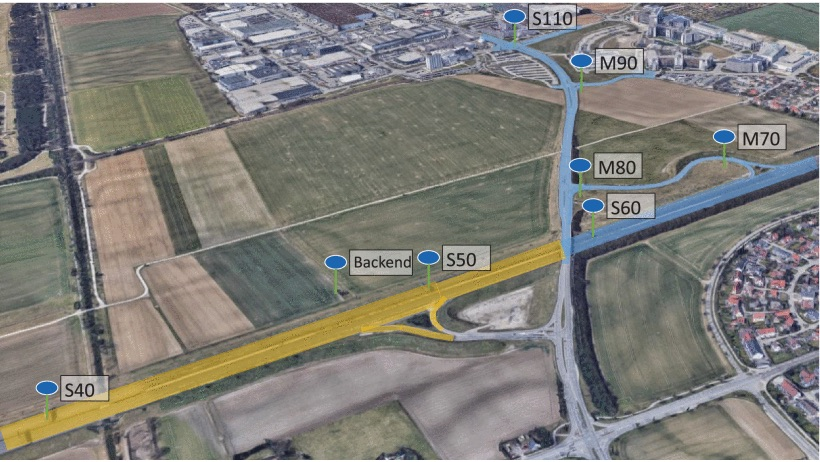
\includegraphics[width=1\textwidth]{providentia_test_bed.jpeg} 
	\caption{Overview of the test bed Providentia++ taken from \cite{a9dataset}. This test bed spans the autobahn A9 and the highway B471 near Munich, covering a total length of 3.5 km}
	\label{fig:providentia_test_bed}
\end{figure}

While highways provide more stable driving conditions for autonomous vehicles, residential areas pose a greater challenge due to their complexity. The transition from highway-centric solutions to residential areas requires innovative approaches and technologies to address the complex and dynamic nature of urban environments. Since 2020, the Providentia project has evolved into Providentia++, led by the Chair of Robotics, Artificial Intelligence, and Real-time Systems at the Technical University of Munich's Department of Informatics. The goal is to extend the deployment beyond highways into encompass residential areas. The addition of Light Detection and Ranging (LiDAR) sensors, along with the existing perception methods, provides redundant road coverage with overlapping fields of view, accurate calibration, and robust detection and data fusion algorithms. The test stretch was expanded into the residential area, enabling the survey of intersections, traffic circles, bus stations, and other urban situations. The complete overview of the Providentia++ test bed is shown in \Cref{fig:providentia_test_bed}

This work is carried out in the scope of the AUTOTech.agil project funded by the Federal Ministry of Education and Research of Germany, which is a continuation of the Prodentia++ project. 

\section{Motivation}

The creation of a digital twin that accurately reflects reality requires precise 3D detection. This crucial task involves building a reliable virtual representation capable of mapping the position, orientation, and dimensions of traffic participants from the real world to the simulator. Previous works in the Providentia project have proposed a Monocular 3D Object Detection (Mono3D) system to generate a three-dimensional digital twin of visible road users from the two-dimensional RGB camera input frames. 

The current system uses YOLOv7 for object detection and has several limitations, such as the inability to classify some classes in the dataset like TRAILER, VAN, EMERGENCY \_VEHICLE, and OTHER. Additionally, it struggles with detecting large or heavily occluded objects, which could impact the final 3D perception and automated driving safety. This thesis aims to enhance the Providentia Mono3D object perception pipeline by predicting real-world 3D object locations and 3D shapes from segmentation masks. 

To achieve this goal, we aim to improve the system's instance segmentation detector. A comprehensive literature review is conducted to identify promising instance segmentation (IS) and amodal instance segmentation (AIS) methods. On the one hand, our approach involves exploring state-of-the-art (SOTA) basic instance segmentation models, outperforming YOLOv7 on the same task. On the other hand, we explore SOTA amodal instance segmentation models that can segment the invisible parts of an object in addition to the visible. We want to investigate whether leveraging amodal segmentation can enhance the system's object detection capabilities, particularly in complex traffic scenarios with significant occlusion.

Moreover, we also explore common datasets with IS and AIS annotations in the domain of autonomous driving for pre-training purposes. Different models are then pre-trained on public autonomous driving datasets and fine-tuned on our TUM Traffic Intersection Extended dataset. Since there are no labeled instance masks in the TUM Traffic Intersection dataset, a subset of frames is annotated for fine-tuning. This enables the models to classify all our categories and learn to predict from our camera settings for improved performance. 

Subsequently, a 2D detector node exploiting these newly trained models is integrated into the existing toolchain. The models are optimized for inference speed using TensorRT. Performance evaluations are conducted, comparing the models against each other and against YOLOv7 in terms of 2D instance segmentation and 3D object detection, utilizing metrics such as Average Precision (AP) and mean Intersection over Union (mIoU).

In essence, this work represents a valuable contribution to the AUTOtech.agil project, effectively addressing the shortcomings of the existing system and potentially advancing the safety and efficacy of autonomous driving technologies.

\section{Contributions}

This thesis presents the following contributions: 

\begin{enumerate}
	\item We explore various state-of-the-art instance and amodal instance segmentation models for inference on the TUM Traffic Intersection dataset. Among these models, we choose the instance segmentation YOLOv8x and the amodal instance segmentation C2F model for further analysis.
	
	\item We propose an instance segmentation labeling pipeline with a method for 2D annotation interpolation across consecutive frames of an image sequence (video). We use this pipeline to extend the TUM Traffic Intersection dataset with visible and full instance segmentation annotations. 
	
	\item We define an extended OpenLABEL annotation structure tailored for our TUM Traffic dataset to include additional modal and amodal segmentation labels. We also extend the TUM Traffic development kit (TUMTraf dev-kit) with label converters facilitating conversion between YOLO, COCO, and our TUM Traffic Dataset OpenLABEL annotation formats. 
	
	\item We leverage YOLOv8x and C2F models pre-trained on COCO and KINS datasets and fine-tuned them on the instance segmentation masks extended frames of the TUM Traffic Intersection dataset. Additionally, we train YOLOv8x from scratch on the extended TUM Traffic Intersection dataset as well as nuImages. 
	
	\item A total of around seven experiments are conducted on the trained models, utilizing different data sequences under various settings to thoroughly evaluate their 2D and 3D perception performance. Notably, the best-performing model for the TUM Traffic Intersection test sequence, across all settings, demonstrates a remarkable 3D mAP@[.10] improvement of 17.79\% compared to YOLOv7, the model currently employed in the Providentia Mono3D system. 
	
	\item We export trained YOLOv8x PyTorch models to TensorRT, resulting in a significant acceleration of inference speed by approximately 2.8 times, surpassing the YOLOv7 TensorRT model's speed by around 2.3 times. Furthermore, we integrate a 2D object detector node, exploiting YOLOv8, into the existing toolchain. 
	
\end{enumerate}


\section{Structure of the Thesis}

The thesis is structured as follows: in \Cref{chap:one}, a comprehensive introduction to the AUTOtech.agil project and its related predecessors is presented, along with the motivation and main contribution of this thesis. \Cref{chap:two} provides an extensive background introduction. This chapter covers the Robot Operating System 1 (ROS1), well-known autonomous driving datasets with instance and amodal instance segmentation annotations, common label formats for object detection tasks, and the labeling tool CVAT. \Cref{chap:three} offers an overview of related works, including the Providentia Mono3D System, followed by an introduction to the state-of-the-art instance segmentation models. \Cref{chap:four} describes in detail the solution approach, including inferencing using different pre-trained models, extending segmentation annotations for the TUM Traffic dataset, training and fine-tuning models, exporting to TensorRT, and integrating into the existing toolchain. \Cref{chap:five} provides an extensive evaluation, including 2D and 3D quantitative analysis, qualitative analysis, as well as an analysis on inference speed, comparing the trained models against the baseline YOLOv7 currently used in the Providentia Mono3D system. \Cref{chap:six} documents five additional experiments on different scenes, including intersection, nighttime, and highway scenarios, with different settings, such as time-shifted ground truth and 3D tracking, to further analyze the generalizability and additional improvements of the proposed models. Finally, \Cref{chap:six} and \Cref{chap:seven} conclude the thesis and suggest avenues for future work.